% Created by tikzDevice version 0.10.1 on 2016-09-05 22:20:49
% !TEX encoding = UTF-8 Unicode
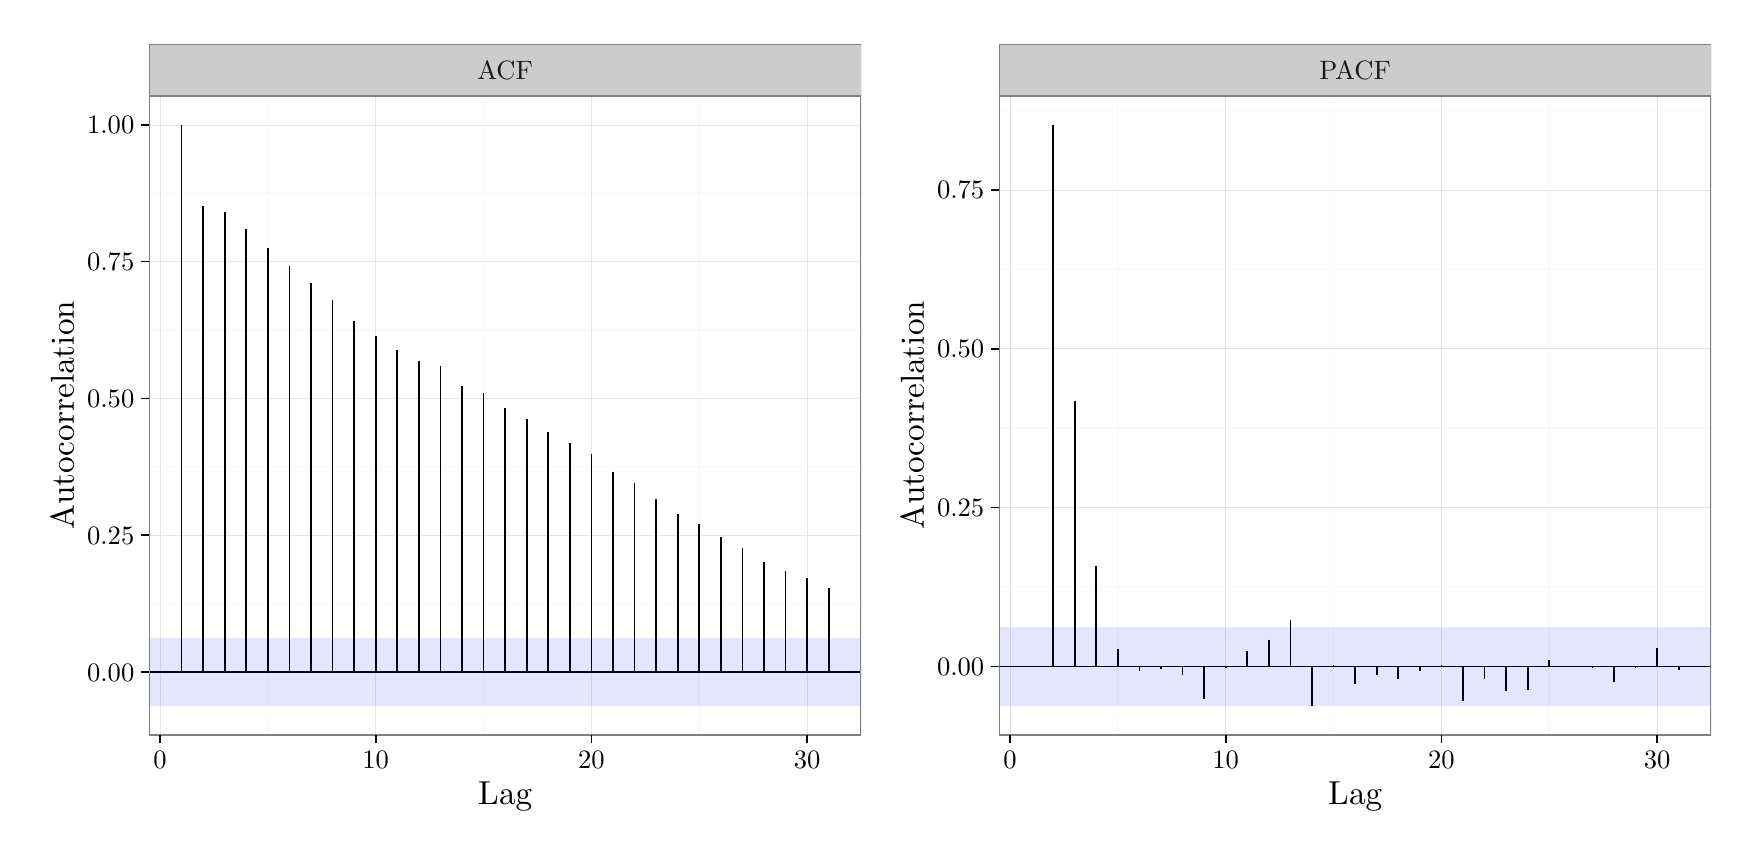
\begin{tikzpicture}[x=1pt,y=1pt]
\definecolor{fillColor}{RGB}{255,255,255}
\path[use as bounding box,fill=fillColor,fill opacity=0.00] (0,0) rectangle (614.29,289.08);
\begin{scope}
\path[clip] (  0.00,  0.00) rectangle (307.15,289.08);
\definecolor{drawColor}{RGB}{255,255,255}
\definecolor{fillColor}{RGB}{255,255,255}

\path[draw=drawColor,line width= 0.6pt,line join=round,line cap=round,fill=fillColor] ( -0.00,  0.00) rectangle (307.15,289.08);
\end{scope}
\begin{scope}
\path[clip] ( 43.93, 33.48) rectangle (301.15,264.47);
\definecolor{fillColor}{RGB}{255,255,255}

\path[fill=fillColor] ( 43.93, 33.48) rectangle (301.15,264.47);
\definecolor{drawColor}{gray}{0.98}

\path[draw=drawColor,line width= 0.6pt,line join=round] ( 43.93, 80.95) --
	(301.15, 80.95);

\path[draw=drawColor,line width= 0.6pt,line join=round] ( 43.93,130.38) --
	(301.15,130.38);

\path[draw=drawColor,line width= 0.6pt,line join=round] ( 43.93,179.82) --
	(301.15,179.82);

\path[draw=drawColor,line width= 0.6pt,line join=round] ( 43.93,229.25) --
	(301.15,229.25);

\path[draw=drawColor,line width= 0.6pt,line join=round] ( 86.80, 33.48) --
	( 86.80,264.47);

\path[draw=drawColor,line width= 0.6pt,line join=round] (164.74, 33.48) --
	(164.74,264.47);

\path[draw=drawColor,line width= 0.6pt,line join=round] (242.69, 33.48) --
	(242.69,264.47);
\definecolor{drawColor}{gray}{0.90}

\path[draw=drawColor,line width= 0.2pt,line join=round] ( 43.93, 56.23) --
	(301.15, 56.23);

\path[draw=drawColor,line width= 0.2pt,line join=round] ( 43.93,105.67) --
	(301.15,105.67);

\path[draw=drawColor,line width= 0.2pt,line join=round] ( 43.93,155.10) --
	(301.15,155.10);

\path[draw=drawColor,line width= 0.2pt,line join=round] ( 43.93,204.53) --
	(301.15,204.53);

\path[draw=drawColor,line width= 0.2pt,line join=round] ( 43.93,253.97) --
	(301.15,253.97);

\path[draw=drawColor,line width= 0.2pt,line join=round] ( 47.82, 33.48) --
	( 47.82,264.47);

\path[draw=drawColor,line width= 0.2pt,line join=round] (125.77, 33.48) --
	(125.77,264.47);

\path[draw=drawColor,line width= 0.2pt,line join=round] (203.72, 33.48) --
	(203.72,264.47);

\path[draw=drawColor,line width= 0.2pt,line join=round] (281.66, 33.48) --
	(281.66,264.47);
\definecolor{drawColor}{RGB}{0,0,0}

\path[draw=drawColor,line width= 0.6pt,line join=round] ( 43.93, 56.23) -- (301.15, 56.23);

\path[draw=drawColor,line width= 0.6pt,line join=round] ( 55.62,253.97) -- ( 55.62, 56.23);

\path[draw=drawColor,line width= 0.6pt,line join=round] ( 63.41,224.75) -- ( 63.41, 56.23);

\path[draw=drawColor,line width= 0.6pt,line join=round] ( 71.21,222.48) -- ( 71.21, 56.23);

\path[draw=drawColor,line width= 0.6pt,line join=round] ( 79.00,216.23) -- ( 79.00, 56.23);

\path[draw=drawColor,line width= 0.6pt,line join=round] ( 86.80,209.37) -- ( 86.80, 56.23);

\path[draw=drawColor,line width= 0.6pt,line join=round] ( 94.59,202.95) -- ( 94.59, 56.23);

\path[draw=drawColor,line width= 0.6pt,line join=round] (102.39,196.99) -- (102.39, 56.23);

\path[draw=drawColor,line width= 0.6pt,line join=round] (110.18,190.64) -- (110.18, 56.23);

\path[draw=drawColor,line width= 0.6pt,line join=round] (117.98,182.92) -- (117.98, 56.23);

\path[draw=drawColor,line width= 0.6pt,line join=round] (125.77,177.69) -- (125.77, 56.23);

\path[draw=drawColor,line width= 0.6pt,line join=round] (133.56,172.72) -- (133.56, 56.23);

\path[draw=drawColor,line width= 0.6pt,line join=round] (141.36,168.80) -- (141.36, 56.23);

\path[draw=drawColor,line width= 0.6pt,line join=round] (149.15,166.79) -- (149.15, 56.23);

\path[draw=drawColor,line width= 0.6pt,line join=round] (156.95,159.47) -- (156.95, 56.23);

\path[draw=drawColor,line width= 0.6pt,line join=round] (164.74,156.91) -- (164.74, 56.23);

\path[draw=drawColor,line width= 0.6pt,line join=round] (172.54,151.58) -- (172.54, 56.23);

\path[draw=drawColor,line width= 0.6pt,line join=round] (180.33,147.57) -- (180.33, 56.23);

\path[draw=drawColor,line width= 0.6pt,line join=round] (188.13,142.97) -- (188.13, 56.23);

\path[draw=drawColor,line width= 0.6pt,line join=round] (195.92,139.03) -- (195.92, 56.23);

\path[draw=drawColor,line width= 0.6pt,line join=round] (203.72,135.10) -- (203.72, 56.23);

\path[draw=drawColor,line width= 0.6pt,line join=round] (211.51,128.58) -- (211.51, 56.23);

\path[draw=drawColor,line width= 0.6pt,line join=round] (219.30,124.53) -- (219.30, 56.23);

\path[draw=drawColor,line width= 0.6pt,line join=round] (227.10,118.64) -- (227.10, 56.23);

\path[draw=drawColor,line width= 0.6pt,line join=round] (234.89,113.28) -- (234.89, 56.23);

\path[draw=drawColor,line width= 0.6pt,line join=round] (242.69,109.71) -- (242.69, 56.23);

\path[draw=drawColor,line width= 0.6pt,line join=round] (250.48,104.93) -- (250.48, 56.23);

\path[draw=drawColor,line width= 0.6pt,line join=round] (258.28,101.00) -- (258.28, 56.23);

\path[draw=drawColor,line width= 0.6pt,line join=round] (266.07, 95.90) -- (266.07, 56.23);

\path[draw=drawColor,line width= 0.6pt,line join=round] (273.87, 92.65) -- (273.87, 56.23);

\path[draw=drawColor,line width= 0.6pt,line join=round] (281.66, 90.10) -- (281.66, 56.23);

\path[draw=drawColor,line width= 0.6pt,line join=round] (289.46, 86.68) -- (289.46, 56.23);
\definecolor{fillColor}{RGB}{0,0,255}

\path[fill=fillColor,fill opacity=0.10] ( 43.93, 43.98) rectangle (301.15, 68.49);
\definecolor{drawColor}{gray}{0.50}

\path[draw=drawColor,line width= 0.6pt,line join=round,line cap=round] ( 43.93, 33.48) rectangle (301.15,264.47);
\end{scope}
\begin{scope}
\path[clip] ( 43.93,264.47) rectangle (301.15,283.08);
\definecolor{drawColor}{gray}{0.50}
\definecolor{fillColor}{gray}{0.80}

\path[draw=drawColor,line width= 0.2pt,line join=round,line cap=round,fill=fillColor] ( 43.93,264.47) rectangle (301.15,283.08);
\definecolor{drawColor}{gray}{0.10}

\node[text=drawColor,anchor=base,inner sep=0pt, outer sep=0pt, scale=  0.96] at (172.54,270.47) {ACF};
\end{scope}
\begin{scope}
\path[clip] (  0.00,  0.00) rectangle (614.29,289.08);
\definecolor{drawColor}{RGB}{0,0,0}

\node[text=drawColor,anchor=base east,inner sep=0pt, outer sep=0pt, scale=  0.96] at ( 38.53, 52.93) {0.00};

\node[text=drawColor,anchor=base east,inner sep=0pt, outer sep=0pt, scale=  0.96] at ( 38.53,102.36) {0.25};

\node[text=drawColor,anchor=base east,inner sep=0pt, outer sep=0pt, scale=  0.96] at ( 38.53,151.79) {0.50};

\node[text=drawColor,anchor=base east,inner sep=0pt, outer sep=0pt, scale=  0.96] at ( 38.53,201.23) {0.75};

\node[text=drawColor,anchor=base east,inner sep=0pt, outer sep=0pt, scale=  0.96] at ( 38.53,250.66) {1.00};
\end{scope}
\begin{scope}
\path[clip] (  0.00,  0.00) rectangle (614.29,289.08);
\definecolor{drawColor}{RGB}{0,0,0}

\path[draw=drawColor,line width= 0.6pt,line join=round] ( 40.93, 56.23) --
	( 43.93, 56.23);

\path[draw=drawColor,line width= 0.6pt,line join=round] ( 40.93,105.67) --
	( 43.93,105.67);

\path[draw=drawColor,line width= 0.6pt,line join=round] ( 40.93,155.10) --
	( 43.93,155.10);

\path[draw=drawColor,line width= 0.6pt,line join=round] ( 40.93,204.53) --
	( 43.93,204.53);

\path[draw=drawColor,line width= 0.6pt,line join=round] ( 40.93,253.97) --
	( 43.93,253.97);
\end{scope}
\begin{scope}
\path[clip] (  0.00,  0.00) rectangle (614.29,289.08);
\definecolor{drawColor}{RGB}{0,0,0}

\path[draw=drawColor,line width= 0.6pt,line join=round] ( 47.82, 30.48) --
	( 47.82, 33.48);

\path[draw=drawColor,line width= 0.6pt,line join=round] (125.77, 30.48) --
	(125.77, 33.48);

\path[draw=drawColor,line width= 0.6pt,line join=round] (203.72, 30.48) --
	(203.72, 33.48);

\path[draw=drawColor,line width= 0.6pt,line join=round] (281.66, 30.48) --
	(281.66, 33.48);
\end{scope}
\begin{scope}
\path[clip] (  0.00,  0.00) rectangle (614.29,289.08);
\definecolor{drawColor}{RGB}{0,0,0}

\node[text=drawColor,anchor=base,inner sep=0pt, outer sep=0pt, scale=  0.96] at ( 47.82, 21.46) {0};

\node[text=drawColor,anchor=base,inner sep=0pt, outer sep=0pt, scale=  0.96] at (125.77, 21.46) {10};

\node[text=drawColor,anchor=base,inner sep=0pt, outer sep=0pt, scale=  0.96] at (203.72, 21.46) {20};

\node[text=drawColor,anchor=base,inner sep=0pt, outer sep=0pt, scale=  0.96] at (281.66, 21.46) {30};
\end{scope}
\begin{scope}
\path[clip] (  0.00,  0.00) rectangle (614.29,289.08);
\definecolor{drawColor}{RGB}{0,0,0}

\node[text=drawColor,anchor=base,inner sep=0pt, outer sep=0pt, scale=  1.20] at (172.54,  8.40) {Lag};
\end{scope}
\begin{scope}
\path[clip] (  0.00,  0.00) rectangle (614.29,289.08);
\definecolor{drawColor}{RGB}{0,0,0}

\node[text=drawColor,rotate= 90.00,anchor=base,inner sep=0pt, outer sep=0pt, scale=  1.20] at ( 16.66,148.97) {Autocorrelation};
\end{scope}
\begin{scope}
\path[clip] (307.15,  0.00) rectangle (614.29,289.08);
\definecolor{drawColor}{RGB}{255,255,255}
\definecolor{fillColor}{RGB}{255,255,255}

\path[draw=drawColor,line width= 0.6pt,line join=round,line cap=round,fill=fillColor] (307.15,  0.00) rectangle (614.30,289.08);
\end{scope}
\begin{scope}
\path[clip] (351.07, 33.48) rectangle (608.29,264.47);
\definecolor{fillColor}{RGB}{255,255,255}

\path[fill=fillColor] (351.07, 33.48) rectangle (608.29,264.47);
\definecolor{drawColor}{gray}{0.98}

\path[draw=drawColor,line width= 0.6pt,line join=round] (351.07, 86.92) --
	(608.29, 86.92);

\path[draw=drawColor,line width= 0.6pt,line join=round] (351.07,144.35) --
	(608.29,144.35);

\path[draw=drawColor,line width= 0.6pt,line join=round] (351.07,201.77) --
	(608.29,201.77);

\path[draw=drawColor,line width= 0.6pt,line join=round] (351.07,259.20) --
	(608.29,259.20);

\path[draw=drawColor,line width= 0.6pt,line join=round] (393.94, 33.48) --
	(393.94,264.47);

\path[draw=drawColor,line width= 0.6pt,line join=round] (471.89, 33.48) --
	(471.89,264.47);

\path[draw=drawColor,line width= 0.6pt,line join=round] (549.84, 33.48) --
	(549.84,264.47);
\definecolor{drawColor}{gray}{0.90}

\path[draw=drawColor,line width= 0.2pt,line join=round] (351.07, 58.21) --
	(608.29, 58.21);

\path[draw=drawColor,line width= 0.2pt,line join=round] (351.07,115.64) --
	(608.29,115.64);

\path[draw=drawColor,line width= 0.2pt,line join=round] (351.07,173.06) --
	(608.29,173.06);

\path[draw=drawColor,line width= 0.2pt,line join=round] (351.07,230.49) --
	(608.29,230.49);

\path[draw=drawColor,line width= 0.2pt,line join=round] (354.97, 33.48) --
	(354.97,264.47);

\path[draw=drawColor,line width= 0.2pt,line join=round] (432.92, 33.48) --
	(432.92,264.47);

\path[draw=drawColor,line width= 0.2pt,line join=round] (510.86, 33.48) --
	(510.86,264.47);

\path[draw=drawColor,line width= 0.2pt,line join=round] (588.81, 33.48) --
	(588.81,264.47);
\definecolor{drawColor}{RGB}{0,0,0}

\path[draw=drawColor,line width= 0.6pt,line join=round] (351.07, 58.21) -- (608.29, 58.21);

\path[draw=drawColor,line width= 0.6pt,line join=round] (370.56,253.97) -- (370.56, 58.21);

\path[draw=drawColor,line width= 0.6pt,line join=round] (378.36,154.28) -- (378.36, 58.21);

\path[draw=drawColor,line width= 0.6pt,line join=round] (386.15, 94.68) -- (386.15, 58.21);

\path[draw=drawColor,line width= 0.6pt,line join=round] (393.94, 64.74) -- (393.94, 58.21);

\path[draw=drawColor,line width= 0.6pt,line join=round] (401.74, 56.71) -- (401.74, 58.21);

\path[draw=drawColor,line width= 0.6pt,line join=round] (409.53, 57.40) -- (409.53, 58.21);

\path[draw=drawColor,line width= 0.6pt,line join=round] (417.33, 55.19) -- (417.33, 58.21);

\path[draw=drawColor,line width= 0.6pt,line join=round] (425.12, 46.39) -- (425.12, 58.21);

\path[draw=drawColor,line width= 0.6pt,line join=round] (432.92, 57.94) -- (432.92, 58.21);

\path[draw=drawColor,line width= 0.6pt,line join=round] (440.71, 63.82) -- (440.71, 58.21);

\path[draw=drawColor,line width= 0.6pt,line join=round] (448.51, 67.85) -- (448.51, 58.21);

\path[draw=drawColor,line width= 0.6pt,line join=round] (456.30, 75.09) -- (456.30, 58.21);

\path[draw=drawColor,line width= 0.6pt,line join=round] (464.10, 44.00) -- (464.10, 58.21);

\path[draw=drawColor,line width= 0.6pt,line join=round] (471.89, 58.84) -- (471.89, 58.21);

\path[draw=drawColor,line width= 0.6pt,line join=round] (479.68, 52.08) -- (479.68, 58.21);

\path[draw=drawColor,line width= 0.6pt,line join=round] (487.48, 55.31) -- (487.48, 58.21);

\path[draw=drawColor,line width= 0.6pt,line join=round] (495.27, 53.67) -- (495.27, 58.21);

\path[draw=drawColor,line width= 0.6pt,line join=round] (503.07, 56.63) -- (503.07, 58.21);

\path[draw=drawColor,line width= 0.6pt,line join=round] (510.86, 58.96) -- (510.86, 58.21);

\path[draw=drawColor,line width= 0.6pt,line join=round] (518.66, 45.90) -- (518.66, 58.21);

\path[draw=drawColor,line width= 0.6pt,line join=round] (526.45, 53.72) -- (526.45, 58.21);

\path[draw=drawColor,line width= 0.6pt,line join=round] (534.25, 49.56) -- (534.25, 58.21);

\path[draw=drawColor,line width= 0.6pt,line join=round] (542.04, 49.82) -- (542.04, 58.21);

\path[draw=drawColor,line width= 0.6pt,line join=round] (549.84, 60.56) -- (549.84, 58.21);

\path[draw=drawColor,line width= 0.6pt,line join=round] (557.63, 58.59) -- (557.63, 58.21);

\path[draw=drawColor,line width= 0.6pt,line join=round] (565.42, 57.59) -- (565.42, 58.21);

\path[draw=drawColor,line width= 0.6pt,line join=round] (573.22, 52.64) -- (573.22, 58.21);

\path[draw=drawColor,line width= 0.6pt,line join=round] (581.01, 58.03) -- (581.01, 58.21);

\path[draw=drawColor,line width= 0.6pt,line join=round] (588.81, 64.85) -- (588.81, 58.21);

\path[draw=drawColor,line width= 0.6pt,line join=round] (596.60, 57.15) -- (596.60, 58.21);
\definecolor{fillColor}{RGB}{0,0,255}

\path[fill=fillColor,fill opacity=0.10] (351.07, 43.98) rectangle (608.29, 72.45);
\definecolor{drawColor}{gray}{0.50}

\path[draw=drawColor,line width= 0.6pt,line join=round,line cap=round] (351.07, 33.48) rectangle (608.29,264.47);
\end{scope}
\begin{scope}
\path[clip] (351.07,264.47) rectangle (608.29,283.08);
\definecolor{drawColor}{gray}{0.50}
\definecolor{fillColor}{gray}{0.80}

\path[draw=drawColor,line width= 0.2pt,line join=round,line cap=round,fill=fillColor] (351.07,264.47) rectangle (608.29,283.08);
\definecolor{drawColor}{gray}{0.10}

\node[text=drawColor,anchor=base,inner sep=0pt, outer sep=0pt, scale=  0.96] at (479.68,270.47) {PACF};
\end{scope}
\begin{scope}
\path[clip] (  0.00,  0.00) rectangle (614.29,289.08);
\definecolor{drawColor}{RGB}{0,0,0}

\node[text=drawColor,anchor=base east,inner sep=0pt, outer sep=0pt, scale=  0.96] at (345.67, 54.91) {0.00};

\node[text=drawColor,anchor=base east,inner sep=0pt, outer sep=0pt, scale=  0.96] at (345.67,112.33) {0.25};

\node[text=drawColor,anchor=base east,inner sep=0pt, outer sep=0pt, scale=  0.96] at (345.67,169.76) {0.50};

\node[text=drawColor,anchor=base east,inner sep=0pt, outer sep=0pt, scale=  0.96] at (345.67,227.18) {0.75};
\end{scope}
\begin{scope}
\path[clip] (  0.00,  0.00) rectangle (614.29,289.08);
\definecolor{drawColor}{RGB}{0,0,0}

\path[draw=drawColor,line width= 0.6pt,line join=round] (348.07, 58.21) --
	(351.07, 58.21);

\path[draw=drawColor,line width= 0.6pt,line join=round] (348.07,115.64) --
	(351.07,115.64);

\path[draw=drawColor,line width= 0.6pt,line join=round] (348.07,173.06) --
	(351.07,173.06);

\path[draw=drawColor,line width= 0.6pt,line join=round] (348.07,230.49) --
	(351.07,230.49);
\end{scope}
\begin{scope}
\path[clip] (  0.00,  0.00) rectangle (614.29,289.08);
\definecolor{drawColor}{RGB}{0,0,0}

\path[draw=drawColor,line width= 0.6pt,line join=round] (354.97, 30.48) --
	(354.97, 33.48);

\path[draw=drawColor,line width= 0.6pt,line join=round] (432.92, 30.48) --
	(432.92, 33.48);

\path[draw=drawColor,line width= 0.6pt,line join=round] (510.86, 30.48) --
	(510.86, 33.48);

\path[draw=drawColor,line width= 0.6pt,line join=round] (588.81, 30.48) --
	(588.81, 33.48);
\end{scope}
\begin{scope}
\path[clip] (  0.00,  0.00) rectangle (614.29,289.08);
\definecolor{drawColor}{RGB}{0,0,0}

\node[text=drawColor,anchor=base,inner sep=0pt, outer sep=0pt, scale=  0.96] at (354.97, 21.46) {0};

\node[text=drawColor,anchor=base,inner sep=0pt, outer sep=0pt, scale=  0.96] at (432.92, 21.46) {10};

\node[text=drawColor,anchor=base,inner sep=0pt, outer sep=0pt, scale=  0.96] at (510.86, 21.46) {20};

\node[text=drawColor,anchor=base,inner sep=0pt, outer sep=0pt, scale=  0.96] at (588.81, 21.46) {30};
\end{scope}
\begin{scope}
\path[clip] (  0.00,  0.00) rectangle (614.29,289.08);
\definecolor{drawColor}{RGB}{0,0,0}

\node[text=drawColor,anchor=base,inner sep=0pt, outer sep=0pt, scale=  1.20] at (479.68,  8.40) {Lag};
\end{scope}
\begin{scope}
\path[clip] (  0.00,  0.00) rectangle (614.29,289.08);
\definecolor{drawColor}{RGB}{0,0,0}

\node[text=drawColor,rotate= 90.00,anchor=base,inner sep=0pt, outer sep=0pt, scale=  1.20] at (323.81,148.97) {Autocorrelation};
\end{scope}
\end{tikzpicture}
